%!TEX root=../../../main.tex

In order to disseminate annotation data in a standardised manner two issues
need to be considered:
\begin{enumerate}
  \item Format annotations using an established specification.
  \item Provide an easy to use mechanism for data distribution.
\end{enumerate}

Regarding the data format, we have chosen the Open Annotation data model, which
recommends using a JSON-LD RDF serialisation for making annotations public
\cite{ref:oa}. Basically, the specification provides a context, in which the
keys are the various OA model components, and the values IRI to various
ontologies, such as FOAF, Dublin Core Metadata Element Set, RDF or the specific
OA vocabulary.

This context can be used by applications to convert their own internal
representations to a standard JSON-LD document; if the internal model is
already in JSON form, this can be achieved directly by compaction or even by
modifying the context keys to match to internal ones.

Despite employing a JSON model in our implementation, we have chosen to
programmatically apply the processing steps. Namely, a thin interface over
JSONAlchemy was implemented\footnote{The code for this wrapper is already
included in the source tree of the next Invenio version and will be shipped
separately from the annotation features.}, allowing objects stored in JSON form
to specify their custom translation method. This method uses a default context,
but custom ones can also be supplied, given that the object class has the
required flexibility.

For the annotations, the method will use the OA context and apply a number of
simple conversions. Let us consider the targeted annotations use-case,
described in Section \ref{sec:notes}, for which the conversions are as follows:
\begin{itemize}
  \item The main identifier of the resource is a IRI pointing to an endpoint of
        the Invenio installation which can supply annotations in the internal
        JSON format; this should not be frequently used, but is included for
        completeness. The type of the resource is \texttt{Annotation} in the
        OA vocabulary.
  \item The OA \texttt{annotatedBy} field is filled with information regarding
        the user that created the annotation. Recall that, internally, we store
        only an identifier, which can be used to retrieve all other associated
        information, such as the name or email address. If, instead of applying
        the explicit conversion process, the JSON-LD compaction routine would be
        used, the mentioned information would need to be directly included in
        the annotation JSON model, resulting in duplication of data. Another
        solution would be to provide only minimal information regarding users,
        namely an IRI pointing to a complete profile\footnote{This is not
        currently available in Invenio.}.
  \item For the \texttt{annotatedAt} field, the time stamp is provided as-is. A
        note here is that, as data producers have no knowledge regarding their
        consumers, time zone information, usually as a value denoting the offset
        from the Coordinated Universal Time (UTC), needs to be included.
  \item For the \texttt{hasBody} field, the annotation content is provided, along
        with its format (\texttt{text/plain}) and encoding (Universal
        Transformation Formats (UTF))
  \item For the \texttt{hasBody} field, the annotation content is provided, along
        with its format (\texttt{format/plain}) and encoding (Universal
        Transformation Formats--8-bit (UTF-8)).
  \item The \texttt{hasTarget} field is encoded as the IRI to the record of the
        document being annotated, along with a OA \texttt{FragmentSelector}
        data type instance, which specifies to what part of the document the
        annotation refers to (a marker such as \textit{``second paragraph on
        third page''}, encoded in the manner described in
        Section \ref{sec:notes}). Note that if a method of accessing document
        fragments directly through a valid IRI is provided, specifying the
        selector is no longer necessary.
\end{itemize}
For annotations on Invenio Web pages the process is similar, except for the
target field, which can be identified uniquely by an IRI. An example of an
expanded JSON-LD representation of a document annotation is included in Fig.
\ref{lst:annojson}.

\begin{figure}[!ht]
  \lstinputlisting[frame=tb,
                   captionpos=b,
                   basicstyle=\footnotesize,
                   numbers=none,
                   showspaces=false,
                   showstringspaces=false,
                   showtabs=false,
                   stepnumber=2,
                   morekeywords={@context,@id,@type,@value},
                   numbersep=4pt]
    {static/lst/rest.json}
    \caption[Expanded JSON-LD document describing an annotation]
            {Expanded JSON-LD document describing an annotation. The internal
             representation is converted to a OA compliant one, using the
             standard vocabulary.}
    \label{lst:annojson}
\end{figure}

Annotation data is served to any interested third-party through a REST Web
interface. At an abstract level, REST is an architectural style in which the
internal system details are ignored, the focus being on the component roles,
the constraints on their interactions, and on the interpretation on significant
data elements.

In terms of Web applications, the REST architecture defines a number of formal
constraints on the client--server communication protocols:
\begin{itemize}
  \item Servers and clients are separated by a uniform interface, each having
        its own distinct set of functions; for example, only servers are
        concerned with data storage, and user interfaces are handled only by
        clients.
  \item Communication is stateless, no client information being stored in the
        server between requests; this requires clients to supply all necessary
        data with each request.
  \item Server responses may be cached and load-balancing may be employed,
        without disrupting clients or corrupting data.
\end{itemize}

The uniform server--client interface is the basis of the REST architecture and
can be described in terms of guidelines regarding the following four aspects:
\begin{enumerate}
  \item Resource identification: resources are uniquely identified (e.g., in Web
                                 applications by IRI) and separated from their
                                 internal structure (e.g., an object stored in a
                                 SQL database will be served to Web clients in a
                                 XML or JSON format).
  \item Resource manipulation: given an object representation, a client holds
                              information to perform any editing or deletion
                              action on the object.
  \item Message description: request responses need to be self-descriptive,
                             specifying the actions clients need to undertake in
                             order to process them. For example, in the case of
                             Web applications, the format of the message (e.g,
                             XML) needs to be included alongside the server
                             response.
  \item Hypermedia as the Engine of Application State (HATEOAS): apart from a
              limited set of simple endpoints, clients do no make any
              assumptions regarding the possible server actions, but follow
              the hyperlinks provided in request responses. For most Web REST
              interfaces, a brief specification defining the endpoints is
              provided, and clients cannot step outside these boundaries,
              except when receiving explicit instructions from the server.
\end{enumerate}

As previously mentioned, the new version of Invenio provides the basic building
blocks for REST interfaces. Each module that desires to implement such an
facility simply needs to define the endpoints, the methods clients can use to
retrieve data (e.g., \texttt{GET} or \texttt{POST}) and the request template.

For the annotation use-case, one endpoint (\texttt{/api/annotations/export}),
accepting two request methods (\texttt{GET} and \texttt{POST}) is provided.
Through the \texttt{GET} method clients can get annotation data in a format
similar to the internal one, this being used, for example, to build the IRI
supplied as the main object \texttt{@id} in the JSON-LD representation (see
Fig. \ref{lst:annojson}). The parameters used for this type of request can be
used to perform simple annotation queries; for example, to retrieve all
annotations targeting the first page of any document a request to
\texttt{api/annotations/export/?where.marker=P.1} can be performed.

More complex queries, along with requests to JSON-LD serialisations can be
performed using the \texttt{POST} method. This allows clients to specify the
request parameters in a JSON document in which three parameters are of interest:
\begin{enumerate}
  \item \texttt{query}: used to filter the retrieved annotations; the format is
                        as defined by MongoDB \cite{ref:mongo}.
  \item \texttt{ldexport}: the JSON-LD format to use for serialisation. Can be
                           \textit{``full''}, which includes the context,
                           expanded, compacted, flattened, framed (having a
                           custom tree structure, see \cite{ref:jsonldframe}),
                           or normalised (RDF triples).
  \item \texttt{new\_context}: the new context to use for compaction or
                               flattening, the tree structure for framing, or
                               the normalisation options (e.g.,
                               \texttt{\{"format": "application/nquads"\}}).
\end{enumerate}

For example, to retrieve the document in Fig. \ref{lst:annojson}, the following
query can be used:
\begin{verbatim}
  curl labs.invenio-software.org/api/annotations/export/  \
       -H "Content-Type: application/json"  \
       --data '{"query": {"where.marker": "P.2-PP.3"},  \
                "ldexport": "compacted",  \
                "new_context": {}}'
\end{verbatim}
Recall that JSON-LD expansion and compaction with an empty context are similar
operations.

The proposed mechanism closely follows the REST guidelines: only a minimal set
of simple, unique, endpoints is provided, clients being allowed to make only
the state transitions specified in the responses (e.g., the main annotation IRI
identifier), responses contain all the information required to perform any
operations over existing annotations and all the responses from the server
contain processing information (the JSON format is advertised on all
responses).  Moreover, the communication is stateless and responses can be
cached as they do not depend on client parameters.

To sum up, Fig. \ref{fig:restanno} provides an overview of the Invenio
annotation system, starting from the end-user interface, through the internal
API, and ending with the REST dissemination service.

\begin{figure}[!ht]
  \centering
  \fbox{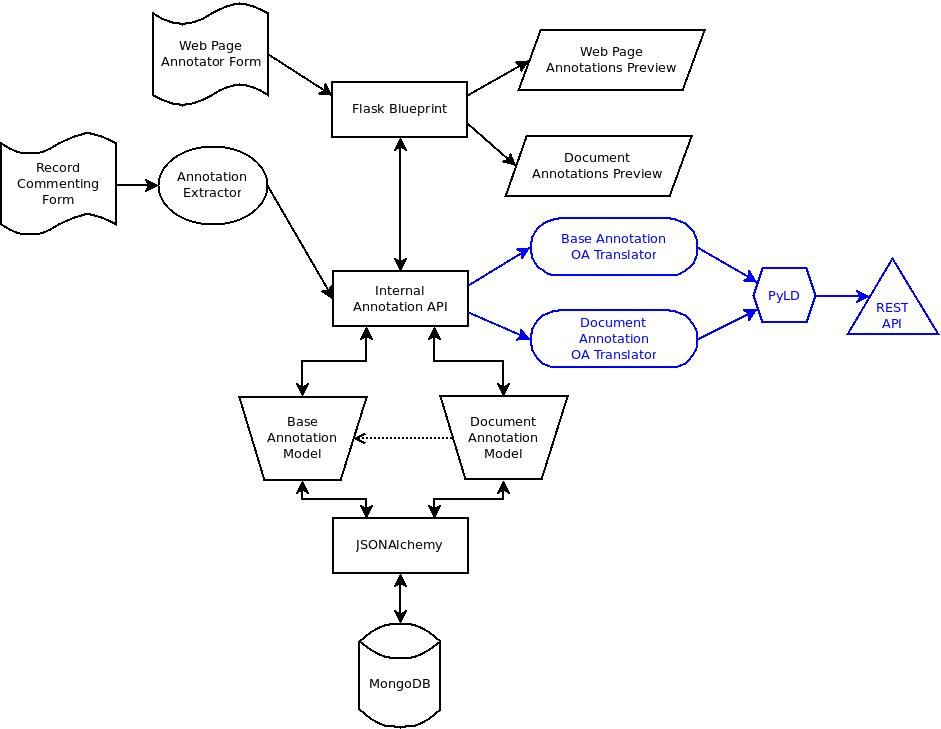
\includegraphics[scale=0.5]{static/dia/rest_anno.jpeg}}
  \caption[Annotation dissemination workflow]
          {Annotation dissemination workflow; after being translated to a proper
           standardised format (Open Annotation JSON-LD) and processed by PyLD,
           user-added annotations can be served by the Invenio REST API to
           concerned third-parties.}
  \label{fig:restanno}
\end{figure}
